\documentclass[a4paper, 14pt]{report}

\usepackage{cmap}
\usepackage[T2A]{fontenc}
\usepackage[utf8]{inputenc}
\usepackage[english,russian]{babel}
\usepackage[left=30mm, top=20mm, right=20mm, bottom=20mm, nohead, nofoot]{geometry}
\usepackage{indentfirst}

\usepackage{amsmath}
\usepackage{MnSymbol}
\usepackage{wasysym}

\usepackage{pgfplots}

\usepackage{tikz}
\usetikzlibrary{graphs}

\usepackage{graphicx}
\graphicspath{{img/}}
\DeclareGraphicsExtensions{.pdf}

\usepackage[most]{tcolorbox}
\newtcolorbox{lbox}[2][] {
    enhanced,
    %fonttitle=\ttfamily,
    %fontupper=\ttfamily,
    sharp corners,
    colback=white,
    colbacktitle=white,
    coltitle=black,
    boxed title style={colframe=white},
    attach boxed title to top center={yshift=-3mm},
    title=#2,#1
}

\author{Гаврилова Юлия Михайловна}
\title{Базы данных}
\date{2019}

\begin{document}
\maketitle

\tableofcontents
\clearpage

\chapter{Введение}

\begin{center}
\begin{tabular}{|c|c|}
    \hline
    \multicolumn{2}{|c|}{Способы организации} \\
    \hline
    \textbf{OLAP} (online analytic processor) & \textbf{OLTP} (jnline transaction processor) \\
    \hline
    Время отклика & Быстрая вставка \\
    \hline
    3NF & 1NF \\
    \hline
    Нормальная форма & Для сбора статистики \\
    \hline
\end{tabular}
\end{center}

\begin{tikzpicture}
    \graph[nodes={align=center,rectangle,draw=black}, grow down sep, branch right sep]
    {
        SQL -> "Reluationnaya model" ->
        {
            "Teoria mnozestv",
            "Teoria predikatov"
        }
    };
\end{tikzpicture}

\hfill

\begin{tikzpicture}
    \graph[nodes={align=center,rectangle,draw=black}, grow down sep, branch right sep]
    {
        SYBD -> BD
    };
\end{tikzpicture}

\section{Реляционная модель}

\begin{enumerate}
    \item Стректурная часть: как построена модель
    \item Целостная часть: какие ограничения, как должны быть организованы данные
    \item Манипуляционная: обработка данных
\end{enumerate}

\subsection{Структурная часть}

\begin{itemize}
    \item Тип int, char
    \item домен - надстройка над типом, набор ограничений/правил (положительные четные для int), можно объявить над типом или над доменом
    \item атрибут - упорядоченная пара (<имя, тип или домен>)
    \item заголовок (схема) отношения - множество всех пар атрибутов \{<имя атрибута$_1$, значение$_1$>,$\dots$, <имя атрибута$_N$, значение$_N$>\}

        \{<$a_1$, int>,<$a_2$, float>,<$a_3$, char>,<$a_4$, varchar>\}
    \item кортеж над схемой

        \{<$a_1$, 1>,<$a_2$, 1.4>,<$a_3$, 'a'>,<$a_4$, 'aaa'>\}
    \item отношение

        \begin{tabular}{|c|c|c|c|}
            \hline
            $a_1$ & $a_2$ & $a_3$ & $a_4$ \\
            \hline
            1 & 1.4 & 'a' & 'aaa' \\
            \hline
        \end{tabular}
\end{itemize}


\paragraph{ER-модель}

\begin{itemize}
    \item отношение/сущность

        \begin{tikzpicture}
            \graph[nodes={align=center,rectangle,draw=black}, grow down sep, branch right sep]
            {
                students -> "second name",
                students -> "group",
                students -> tails,
                students -> number
            };
        \end{tikzpicture}
\end{itemize}

Здесь студент сущность сильная. Если студент зависит, то студент - слабая сущность

\begin{itemize}
    \item связь 1 - 1 (Студент $\to$ зачетка)
    \item связь 1 ко многим (Студенты $\to$ группа)
    \item многие ко многим (Студенты $\to$ курс)
\end{itemize}

\begin{lbox}{\textbf{Лабораторная работа 1}}
    \begin{itemize}
        \item Подобрать предметную область на весь семестр
        \item ER модель (не менее 3ч самостоятельных сущностей)
        \item Создать свою БД (не менее 1000 записей на таблицу)
    \end{itemize}
    \textbf{Защита:}
    \begin{itemize}
        \item Добавить связь/атрибут
        \item Создать ссылку
    \end{itemize}
\end{lbox}

\subsection{Целостная часть}

\begin{itemize}
    \item целостность сущностей/отношений
    \item целостность ссылок

        \begin{tabular}{|c|c|c|}
            \hline
            id & ФИО & Age \\
            \hline
            1 & Иванов & 10 \\
            \hline
            2 & Петров & 15 \\
            \hline
            3 & Иванов & 45 \\
            \hline
        \end{tabular}
\end{itemize}

Потенциальный ключ:

\begin{itemize}
    \item однозначная идентификация записи
    \item никаких подмножеств не должно быть под ключом
\end{itemize}

\begin{center}
    \begin{tabular}{|c|c|c|}
        \hline
        id & ФИО & id группы \\
        \hline
        1 & Петров & 1 \\
        \hline
        & & \\
        \hline
    \end{tabular}

    $\downarrow$ Внешняя ссылка

    \begin{tabular}{|c|c|}
        \hline
        id & Название \\
        \hline
        1 & ИУ7-53 \\
        \hline
        & \\
        \hline
    \end{tabular}
\end{center}

Ссылочная целостность - нельзя ссылаться на несуществующий объект

\subsection{Манипуляционная часть}

\begin{itemize}
    \item Реляционная алгебра
    \item Реляционные исчисления
\end{itemize}

\section{Реляционная алгебра}

\begin{tabular}{|c|c|}
    \hline
    id & name \\
    \hline
    1 & a \\
    \hline
    2 & b \\
    \hline
\end{tabular}

\hfill

\begin{tabular}{|c|c|}
    \hline
    id & name \\
    \hline
    2 & b \\
    \hline
    3 & c \\
    \hline
\end{tabular}

\begin{enumerate}
    \item Традиционные - работа с множеством

        \begin{itemize}
            \item Объединение (UNION)

                \begin{tabular}{|c|c|}
                    \hline
                    id & name \\
                    \hline
                    1 & a \\
                    \hline
                    2 & b \\
                    \hline
                    3 & c \\
                    \hline
                \end{tabular}

            \item Пересечение (INTERSECT)

                \begin{tabular}{|c|c|}
                    \hline
                    id & name \\
                    \hline
                    2 & b \\
                    \hline
                \end{tabular}

            \item Вычитание (MINUS)

                \begin{tabular}{|c|c|}
                    \hline
                    id & name \\
                    \hline
                    1 & a \\
                    \hline 
                \end{tabular}

                \begin{tabular}{|c|c|}
                    \hline
                    id & name \\
                    \hline
                    3 & c \\
                    \hline 
                \end{tabular}

            \item Декартово произведение (TIMES) - все возможные комбинации атрибутов
        \end{itemize}

    \item Специальные

        \begin{itemize}
            \item Соединение (JOIN)

                \begin{tabular}{|c|c|c|}
                    \hline
                    id & name1 & name2\\
                    \hline
                    2 & b & b \\
                    \hline
                \end{tabular}

            \item Ограничение (WHERE)
            \item Проекция (PROJECT)
            \item Деление (DIVIDE BY)
        \end{itemize}
\end{enumerate}

Реляционное выражение = унарное выражение (бинарное выражение)

\paragraph{Унарные выражения}

\begin{itemize}
    \item Проекция

        терм | терм[список атрибутов]

    \item Ограничение

        терм WHERE логическое\_выражение

    \item Переименование

        терм RENAME old\_name TO new\_name

\end{itemize}

терм - имя\_отношения | (реляционное\_выражение)

\paragraph{Бинарные выражения}

\begin{itemize}
    \item Объединение
    \item Пересечение
    \item Вычитание
    \item Декартово произведение
    \item Соединение
\end{itemize}

бинарные операции = проекция бинарная\_операция реляцонное\_выажение

S JOIN P[P..,S..]

\begin{tabular}{|c|}
    \hline
    Поставщик \\
    \hline
    S \\
    \hline
\end{tabular}

$ \downarrow $ Многие ко многим SP

\begin{tabular}{|c|}
    \hline
    Детали \\
    \hline
    P \\
    \hline
\end{tabular}

\hfill

$S(Sno : integer, Sname : string, Status : integer, City : string)$

$P(Pno : integer, Pname : string, Color : string, Weight : real, City : string)$

$SP(Sno : integer, Pno : integer, Quantity : integer)$

\paragraph{S}

\hfill

\begin{tabular}{|c|c|c|c|}
    \hline
    Sno & Sname & Status & City \\
    \hline
    1 & Алмаз & 20 & Смоленск \\
    2 & Дельта & 10 & Владимир \\
    3 & Орион & 30 & Смоленск \\
    \hline
\end{tabular}

\paragraph{P}

\hfill

\begin{tabular}{|c|c|c|c|c|}
    \hline
    Pno & Pname & Color & Weight & City \\
    \hline
    1 & Гайка & К & 12.0 & Смоленск \\
    2 & Болт & С & 17.1 & Рязань \\
    3 & Винт & З & 15.47 & Владимир \\
    4 & Винт & К & 18 & Москва \\
    5 & Шайба & З & 25 & Смоленск \\
    \hline
\end{tabular}

\paragraph{SP}

\hfill

\begin{tabular}{|c|c|c|}
    \hline
    Sno & Pno & Quantity \\
    \hline
    1 & 1 & 25 \\
    1 & 2 & 14 \\
    2 & 4 & 2 \\
    \hline
\end{tabular}

\begin{enumerate}
    \item Имена всех поставщиков детали под номером 2

        $$
        \underbrace{((\underbrace{\text{SP join S})}_\text{рел. выр.} \text{where} \underbrace{\text{Pno = 2}}_{\text{лог. выр.}})}_\text{реляционное выражение}[\text{Sname}]
        $$

        select Sname

        from SP inner join S on SP.Sno = S.Sno

        where SP.Pno = 2

    \item Вывести все имена поставщиков, которые поставляюк как минимум одну красную деталь

        $$
        (((\text{P where } \text{Color = 'К'}) \text{join SP}) \text{join S})[\text{Sname}]
        $$

    \item Получить имена поставщиков, которые поставляют все детали

        $A(X_1, \dots, X_n, Y_1, \dots, Y_n)$

        $B(Y_1, \dots, Y_n)$

        $A \text{ divide by } B = (X_1, \dots, X_n)$

        \begin{tabular}{|c|c|}
            \hline
            Sno & Pno \\
            \hline
            1 & 1 \\
            1 & 2 \\
            1 & 3 \\
            2 & 2 \\
            2 & 3 \\
            3 & 1 \\
            \hline
        \end{tabular}

        $P[Pno]$

        $SP \text{ divide by } P[Pno]$

        $((SP \text{ divide by } P[Pno]) \text{ join } S)[Sname]$

    \item Все поставщики, которые поставляют только красные детали

        $(Sp \text{divide by }(P \text{ where } \text{Color = 'К'})[Pno])[Sname]$

    \item Переименовать города из первой таблицы во вторые

        $(S \text{ rename } Sno \text{ to } firstName)[firstName, City] \text{ join }$
        
        $(S \text{ rename } Sno \text{ to } secondName)[secondName, City]) \text{ where } secondName > firstName \text{ join } S$

        \begin{tabular}{|c|c|}
            \hline
            firstName & C \\
            \hline
            1 & С \\
            2 & В \\
            3 & С \\
            \hline
        \end{tabular}

        \begin{tabular}{|c|c|}
            \hline
            secondName & C \\
            \hline
            1 & С \\
            2 & В \\
            3 & С \\
            \hline
        \end{tabular}

        \begin{tabular}{|c|c|c|}
            \hline
            firstName & secondName & C \\
            \hline
            1 & 1 & С \\
            1 & 3 & С \\
            2 & 2 & В \\
            3 & 1 & С \\
            3 & 3 & С \\
            \hline
        \end{tabular}

    \item Поставщики, которые не поставляют деталь номер 2

        $((S[Sno] \text{ minus } (SP \text{ where } Pno=2)[Sno]) \text{ join } S)[Sname]$

\end{enumerate}

\subsection{GROUP}

SP group (Pno, Qty) as PQ - группирует

\begin{tabular}{|c|c|c|}
    \hline
    Sno & Pno & Qty \\
    \hline
    1 & 1 & 10 \\
    \hline
    1 & 2 & 15 \\
    \hline
    2 & 1 & 5 \\
    \hline
\end{tabular}

$\downarrow$

\begin{tabular}{|c|c|}
    \hline
    Sno & PQ \\
    \hline
    1 & 1-10 2-15 \\
    \hline
    2 & 1-5 \\
    \hline
\end{tabular}

\subsection{Summarize}

summarize SP per SP \{Pno\} add sum(Qty) as sQty

\begin{tabular}{|c|c|}
    \hline
    Pno & sQty \\
    \hline
    1 & 15 \\
    \hline
    1 & 16 \\
    \hline
\end{tabular}

extend S add 'Поставщик' as Sname2

extend SP add Qty*100 as Qty2

\subsection{UNGROUP}

\section{Реляционное сравнение}

S(Sno) = SP(Sno)

is\_epmty(реляционное выражение)

t in R $\Leftrightarrow$ RELATION\{t\} $\le$ R

t - Кортеж

R - отношение

\begin{center}
    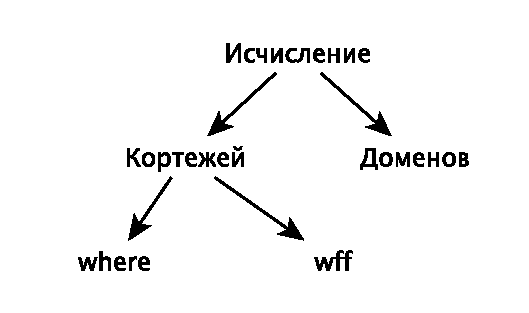
\includegraphics{db1}
\end{center}

объявление = range of переменная is список

область = отношение | реляционное выражение

реляционное выражение = (список целевых элементов) [where(wff)]

целевой элемент = переменная | переменная атрибут [as имя]

wff = условие | not условие | условие and (or) wff | if условие then(wff)

\paragraph{Примеры}

\hfill

range of SX is S

range of SPX is SP

range of SY is (SX) where SX.City = 'Смоленск', (SX) where exists SPX(SPX.Sno=SX.Sno and SPX.Pno=1)

Задачи как в реляционной алгебре

\begin{enumerate}
    \item range of SX is S (SPX.Sno) where SPX.Pno = 2 (SX.Sname) where exists SPX(SPX.Sno = SX.Sno and SPX.Pno = 2)
    \item range of SX os P (SX.Sname) where exists SPX(SPX.Sno = SX.Sno and exists PX(SPX.Pno = PS.Pno and PX.Color = 'К'))

        (SX.Sname) where exists SPX(where exists PX(SPX.Sno = SX.Sno and SPX.Pno = SX.Pno and PX.Color = 'к'))

        range of PX is (Pno) where P.Color = 'К'

    \item (SX.Sname) where forall PX(exists SPX(SPX.Pno = SX.Pno and SPX.Sno = SX.Sno))

    \item <$S_1$, $S_2$>

        range of SY is S (SX.Sname as FirstName, SY.Sname as SecondName) SX.City = SY.City and SX.Sno > SY.Sno

    \item (SX.Sname) where not exists SPX(SPX.Sno = SX.Sno and SPX.Pno = 2)
\end{enumerate}

\subsection{Агрегатные сравнения}

(sum(SPX.Qty) as Total)

агрегатная функция((атрибуты) where f[атрибуты])

\end{document}
